\section{Planning and execution in the \texttt{T-REX} architecture}
\label{sec:arch}

\subsection{The T-REX architecture}
\label{sec:arch:trex}


{\em This section presents quickly T-REX architecture but move
  quickly the focus on a single reactor and gross concepts on the
  architecture:
  \begin{itemize}
  \item For t-trex the whole decision and control problem is reduced
    around the state variables (or timeline construct). 
  \item This reduce the execution tracking problem for each reactor on a state
    identification problem (deduce internal state from the external
    state), and the control problem to goal posting which will trigger
    deliberation on the owner of the corresponding timeline. 
  \item the architecture itself see each reactor as a black box and
    therefore each reactor can implement its own mechanism in order to
    resolve both synchronization and deliberation. Still we provide a
    reactor based on the europa framework that leverage the automated
    planning capabilities in order to do model based planning and
    execution with a rich representation of resources and time.
  \end{itemize}}


\subsection{The Europa deliberative reactor}
\label{sec:arch:europa}

In T-REX architecture reactors have two core functions;
synchronization where the main focus is to track and refine the
evolution of the state of the world at any single tick, and
deliberation which focus on providing a plan to the agent in order to
complete the reactor {\em Internal} goals. These two processes are
intertwined in the sense that one influences the outcome of the
other. They are represented as two europa solvers modifying the same
plan database and for which the execution is managed by the T-REX 
framework rythemed by the time advance during the execuion of the
system:
\begin{enumerate}
\item The synchronization solver is a specialized eurpa solver that
  will integrate in the plan new information about the evolution of
  the External state varaible and ensure that the reactor propagate
  these in order yto both identify its current stetate and inform
  other reactors of any state change on its internal timelines. This
  solver is summoned at the beginnning of every single tick.
\item The deliberation solver is managing the deliberation process of
  the reactor in order to produce a new plan or alter its current plan
  as new goals are given to the reactor or the synchronization solver
  identifying a conflict between the current state of the world and
  the expectations of the previous plan. This process can  span other
  multiple tick and therrfore can be interrupted at any single tick in
  order for the synchronization solver to do its task.
\end{enumerate}

In  this section we present how both processes are implemented using
the europa framework. We first present each of them independently by
looking to their specific focus. We then develop how both processes
are not only interleaved (as deliberation can take several tick while
synchronization eneds to happen at every single tick) but also discuss
on how each of these is impacting the other and how this intertwining 
of the two result on an emergent behavior of the reactor by allowing
the system to efficiently adapts its plan that can then be dispatched
as objectives for the reactors it depends on in a seamless flow. 

\subsubsection{Synchronization identify internal state evolution}
\label{sec:arch:synch}

For the sake of simplicity we introduce first how a reactor can track
and identify its state in the context where it does not have any
compelling need to deliberate. Assume here that we have a reactor that
have no future goal. {\em Need to develop the reason why it is a
  necessity: primarily to provide its internal state to whoever
  observe it but als simply to ensure that its current representation
  of the world is up to date and still consistent}

In the europa based reactor we introduce this requirement as a new
type of flaw for the europa framework. This flaw enforces at the
reactor to identify fully its internal state for the current
tick. By using this new flaw we can describe the synchronization
process as this general sequence :
\begin{enumerate}
\item Integrate the external state as provided by the owner of each
  external timeline into the plan database.
\item Propagate this information in the plan database following the
  model $\mathcal{M}$ of this reactor.
\item Resolve the current state value of each internal timelines.
\end{enumerate}

\begin{figure}[!htbp]
  \centering
  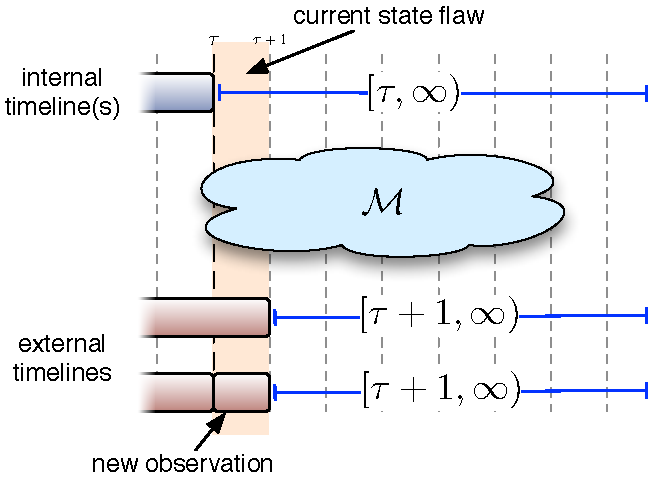
\includegraphics[width=0.5\columnwidth]{figs/synch-relation}
  \caption{Ilustration of the synchronization flaws in a reactor. The
    reactor receive new observations when they are produced by the
    owner(s) of its internal timelines. The line after the last token
    of each timeline represent the domain of possible values for the
    end of this token. At every tick $\tau$ the reactor needs to
    integrate the {\em External} state information it received and --
    based on its model $\mathcal{M}$ -- resolve its {\em Internal}
    state that will then be provided by the architecture to other
    reactors using these state variables.}
  \label{fig:synch:flaw}
\end{figure}

The resolution of internal state flaw can be resolved using one of the
following choices which are evaluated in the given order:
\begin{enumerate}
\item Extend the previous state value to end after this tick (ie
  restrict its end time to $[\tau+1, \infty)$). 
\item Start the next active token in the timeline and
  attempt to start it now (ie restrict its start time to the single
  value $\tau$).
\item Create and insert a new token in this timeline that will start
  at the current tick $\tau$ (attempt this for each possible token
  type for this timeline if necessary). 
\end{enumerate}

All of these choices are evaluated sequentially until a consistent
solution with no more flaw for this tick is identified. In order to do
so we need to make the assumption that the current state value of an
internal timeline do not depend on the future or more accurately
that any choices made during this synchronization will not lead to a
future inconsistency (meaning no possible solution) for a future
synchronization. Such assumption deeply impact the set of possible
domains one the reactor can support while remaining complete. Take for
example the following model rule where {\tt Vehicle} is {\em Internal}
and {\tt Command} is {\em External} to the reactor.
\begin{verbatim}
Vehicle::Dive {
  contains(Command.Descend descend);
  descend.start = start + 2;
}
\end{verbatim}

Such model present the issue that the reactor needs at one point to
take the decision to start the token {\tt Vehicle.Dive} and by doing
so it assumes that in {\em exactly} 2 ticks in the future the {\tt
  Command} timeline will change its state to {\tt Command.Descend}. If
this observation does not occur at the given time this implies that
the reactor estimation was wrong leading him to an inconsistent view
of the world. Conversely the reactor can decide to not switch this
timeline to the {\tt Vehicle.Dive} state and observe 2 ticks in the
future that the {\tt Command.Descend} state value. In this case it
would have missed the opportunity to set its {\tt Vehicle} state to
the correct value which may similarly lead (depending on the rest of
the model) to a similar inconsistency it won't be able to resolve (as
TREX enforces that  the past is monotonic).

While this limitation of the system is important to take into account,
it is also important to note that the model snippet we gave here --
while formally acceptable in the general planning problem -- is also
illustrating a bad design for execution in a situated agent. Indeed,
in this model we are tying the current decision to a future outcome
that is {\em External} to the reactor and therefore not necessarily
controllable by this reactor. Therefore we are entailing a part of the
future to past decisions which can lead the system to a dead-end
situation where the model cannot find a correct solution that both do
not conflict with what we claimed in the past and still allow the
planner to find its current {\em Internal} state.


\subsubsection{Deliberation : planning for future state evolution}
\label{sec:arch:plan}




\subsubsection{Intertwining synchronization and execution }
\label{sec:arch:intertwine}




% Gives a high-level overview of T-REX, the general design principles and how
% these principles aid in software engineering. Show T-REX block diagram.



%%% Local Variables: 
%%% mode: latex
%%% TeX-master: "setobook"
%%% End: 
